
\documentclass[11pt]{memoir} % use larger type; default would be 10pt


%inkluderte pakker
\usepackage[utf8]{inputenc}
\usepackage{hyperref}
\usepackage{paralist}
\usepackage{graphicx}
\usepackage[margin=8pt,font=small,labelfont=bf]{caption}

%slutt på pakkene

\title{- Prosjektoppgave - \\ Samfunnsmedisinkurs C \\ Oslo, 11.- 13. November 2013}
\author{Pål Ager-Wick \\ Kommuneoverlege Øvre- og Nedre Eiker}
\date{} % Activate to display a given date or no date (if empty),
         % otherwise the current date is printed 

\begin{document}
%%Her begynner oversettelsen til norsk
			\renewcommand{\chaptername}{Del}
            \renewcommand{\contentsname}{Innhold}
            \renewcommand\listfigurename{Illustrasjoner}
            \renewcommand\tablename{Tabell}
			\renewcommand\listtablename{Tabeller}
            \renewcommand{\figurename}{Illustrasjon}

%%Her slutter den
\frontmatter

\maketitle

\chapter{Forord til oppgaven}
	Jeg skriver her et kort forord fordi jeg har langt overskredet sidetallet som var satt til to sider. Det er i størst grad fordi jeg velger å skrive dokumenter i et spesielt format som gjør dem mer leservennlige og lettere å disponere når man skal skrive. Jeg tror derfor at oppgaven, selv om den er på betydelig mer enn to sider, likvel vil tilsvare omlag 2 tettskrevne A4 sider.\\

	Denne programvaren er åpen. Dette standarden for innleveringer av oppgaver ved for eksempel Universitet i Oslo. Dersom det er mer interesse kan man gjøre et google søk etter LaTex, som er et programmeringsspråk som kompileres til portable datafiler(pdf).\\

	Det finnes en fullstendig versjonsoversikt som er åpent tilgjengelig på \href{http://pcjawick.github.io/Folkehelseoppgave}{GitHub}. Her kan du laste ned hele prosjektet og finne lenke til versjonsoversikten.\\

	Til slutt tillater jeg meg en tilbakemelding om at denne oppgaveteksten, som i seg selv var på 1/2 A4 side, vanskelig kan komme under 2 A4 sider på en meningsfull måte.\\[1in]



DRAMMEN 26.10.2013\\[0.5in]

Pål CJ Ager-Wick

\newpage

\tableofcontents

\mainmatter

\chapter{Utfordringer for Nedre Eiker kommune}
	\section{Folkehelseprofilen}
		\paragraph{}
			Som tidligere allmennlege tok det tid før folkehelsebegrepet ble konkret for meg. Som så ofte med begrep som favner mange samfunnsområder og er vanskelige å definere med få ord, strøs "Folkehelse" omkring som et prydord i taler og slagord i valgkamper. Da vi fikk folkehelseprofilene i 2012 kom bakkekontakten og derfor velger jeg å begynne der.  
%Her begynner grafikken

                    \begin{figure}[ht]
                      \centering
                      	\frame{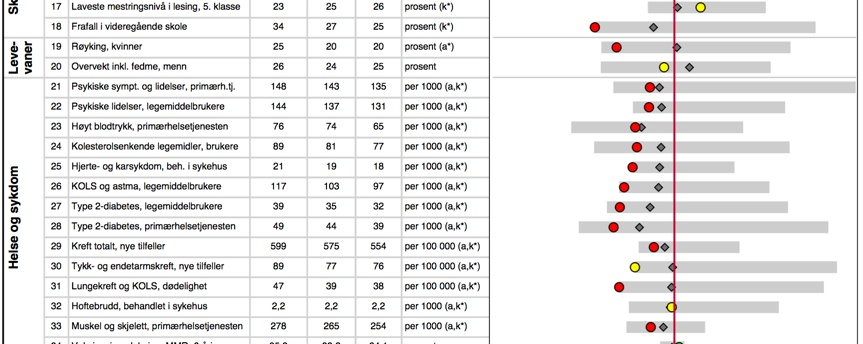
\includegraphics[width=4.4in]{./fhprofilnek.jpg}}%utklipp fra fh profilen 2013
                      \captionsetup{singlelinecheck=off}
                      \caption{Utdrag fra folkehelseprofilen i Nedre Eiker}
                      {Figuren viser et utdrag fra folkehelseprofilen i Nedre Eiker. Her er det mye å ta fatt i, men det skyldes det selektive utsnittet. Jeg ønsker å vise at folkehelseprofilen kan være vanskelig å bruke som datagrunnlag med et så mangfoldig problemområde. Omvendt kan de positive trendene være falsk positive av på grunn av metodene eller befolkningssammensetningen.\cite{fhprofil}}\label{fhprofilnekbilde}%\textit{tjenestetilbudene}.]
                    \end{figure}    

%Her slutter grafikken
		
	\section{Eksisterende planverk}
		\paragraph{}
			Det er viktig å danne seg et bilde av eksisterende planverk og hvilke tiltak som allerede jobber inn mot samme område. Det har gått lang tid siden Ottawa charteret\cite{ottawa} ble skrevet, men de grunnleggende elementene forblir de samme. De grunnleggende behovene for helse er like gyldige i dag og er i stor grad integrert i internasjonal politikk. Det er blitt etablert at mat, husly, utdannelse og fred er universelle suksessfaktorer for å kunne være et suksessrikt samfunn, men også for god livskvalitet. Og ved stikkordet livskvalitet er vi kommet til måleenheten for folkehelsearbeid, og kanskje også vnalig helsearbeid.\\
		\paragraph{}
			I vår kommune jobbes det for tiden med en folkehelseplan slik det er beskrevet i folkehelseloven\cite{Folkehelseloven}. Her er arvematrialet fra Ottawa charteret\cite{ottawa} godt synlig, med tverfaglig jobbing som et sentralt tema. 

			  \begin{figure}[h]
                      \centering
                      	\frame{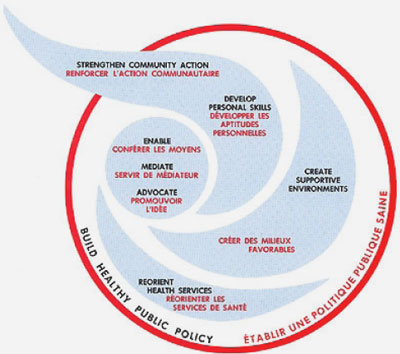
\includegraphics[width=4in]{./hpr_logo}}%utklipp fra fh profilen 2013
                      \captionsetup{singlelinecheck=off}
                      \caption{Arbeidsprinsipp fra Ottwacharteret}
                      %\textit{tjenestetilbudene}.]
                    \end{figure}   
        \paragraph{}
        	I vårt planverk har vi i dag flere planer som sneier innom folkehelsearbeid. Folkehelsearbeidet skal jo være tverrfaglig og "i alt vi gjør", men forløpig er det lite helt håndfast. Vår største satsing er i samarbeid med nabokommunen med frisklivssentralen "Aktiv Eiker". Disse driver folkehelsearbeid med kommunens befolkning hver dag og er blitt synonymt med folkehelse i kommunen. Utfordringer er å flytte fokuset videre utover alle de kommunale tjenestene.

	\section{Hvordan virkeligheten ser ut}
		\paragraph{}
			- Folkehelsen i Norge er bedre en noen gang, innleder rapporten om utviklingstrekk i folkehelsearbeidet\cite{Utvtrekk}. Likevel er det tydelig å lese at vi ikke lykkes i arbeidet med å utjevne sosiale forkjeller. Dette medfører forkjeller i levealder og livskvalitet som kanskje kunne vært endret dersom vi legger forholdene til rette. Jeg vil ta en liten politisk ekskursjon før jeg kommer tilbake til Nedre Eikers virkelighet.

		\paragraph{}
			Her ligger noe av utfordringen slik jeg ser det: Det er mye politikk i folkehelsearbeidet, særlig på den internasjonale arena. I dagens politiske klima er egalitetstankegangen utfordret av liberalismen. Finanskrisens etterspill er gode eksempler på det, med systematisk nedbygging av det offentlige. Samtidig uthules det statlige finansapparatet med "Quantitative easing", et begrep som brukes om statens evne til å trykke penger for å motvirke markedenes reduserte verdi. Disse makroøkonomiske mekanismene utgjør en stor og reel trussel mot folkehelsa i Europa og også indirekte Norge.

		\paragraph{}
			Nedre Eikers problemområder er gjengitt på side \pageref{fhprofilnekbilde}. Oppsummert har vi de største utfordringene innen helse og levevaner. Jeg vil i \nameref{chap:fok} gå nærmere inn på hvordan jeg mener man kan arbeide systematisk og tverrfaglig med dette. 

\chapter{Fokusområde: Fysisk helse}\label{chap:fok}
	\section{Hvorfor fysisk helse?}
		\paragraph{}
			Den mest effektive måten å bekjempe dårlige levevaner og de fleste sykdommer er å få flere i aktivitet\cite{aktivhb}. Dette er et uttalt mål fra Folkehelsinstituttet(FHI)\cite{htnorge} at alle skal være en time mindre inaktive hver dag. Det er mye forskning som tyder på at dette vil være ekstremt gunstig og samtidig billig\cite{aktivhb}.
					\begin{figure}[h]
                      \centering
                      	\frame{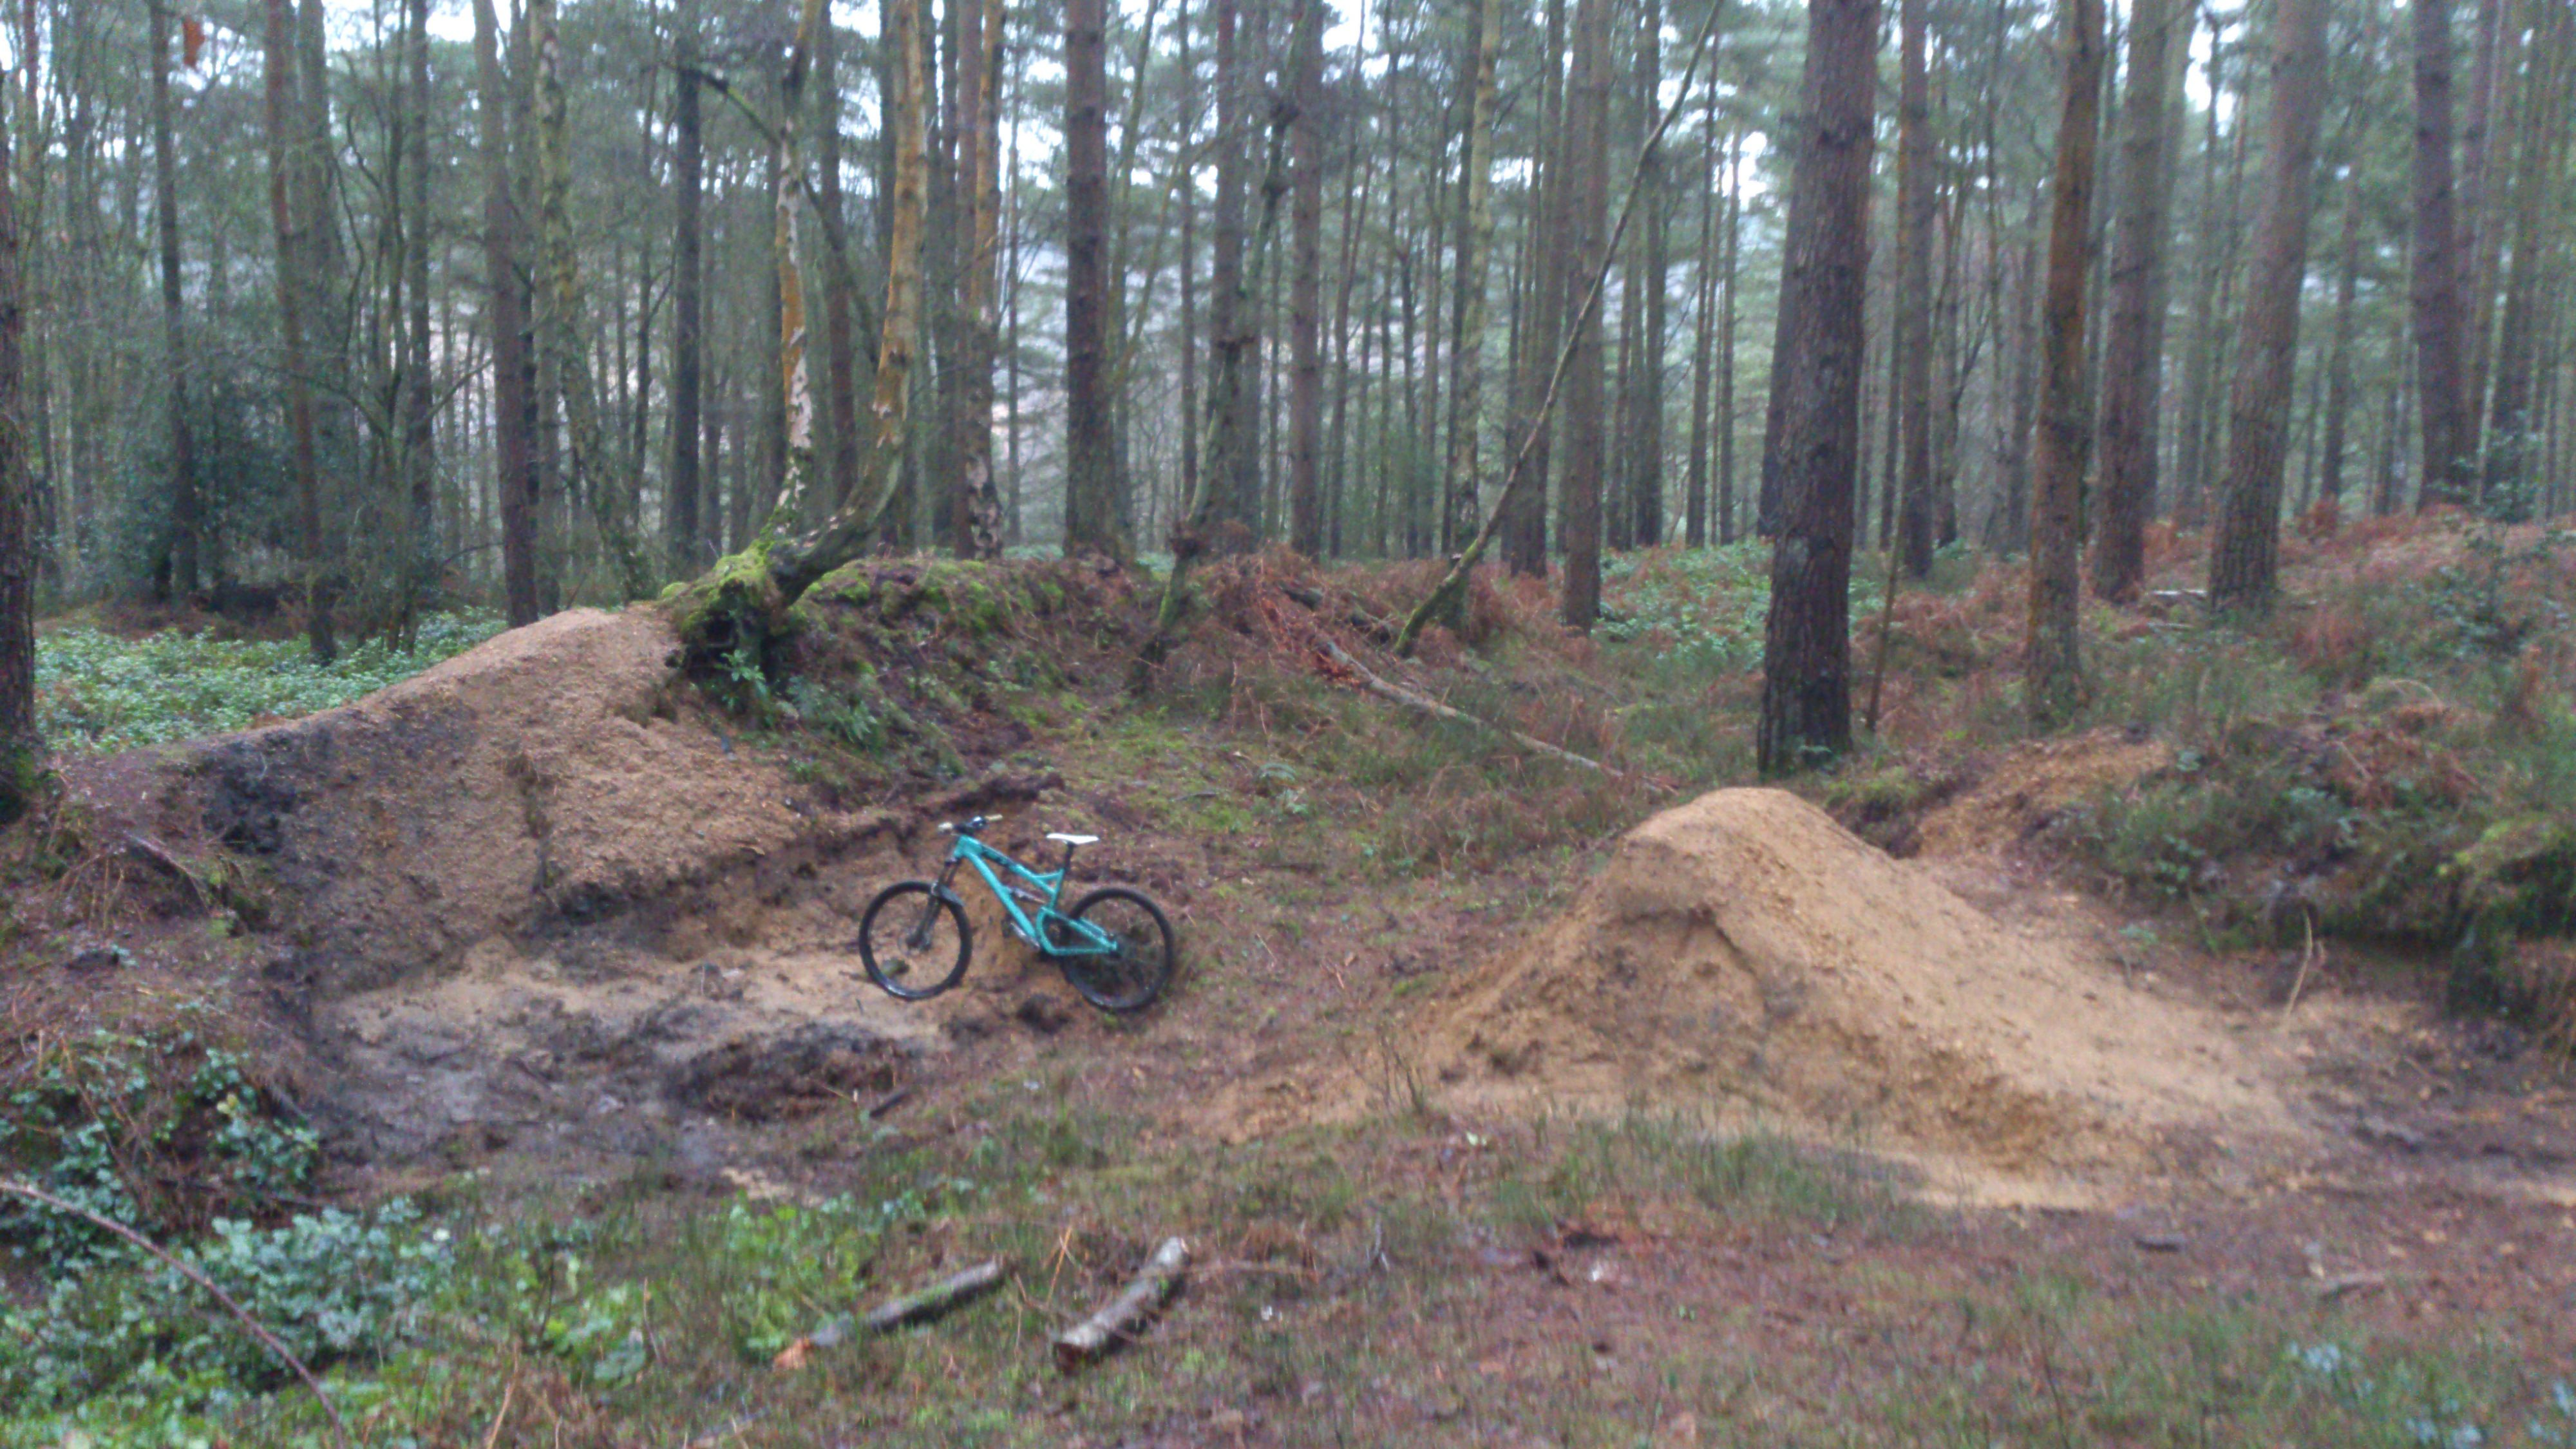
\includegraphics[width=4.5in]{./bikeuk}}%utklipp fra fh profilen 2013
                    	  \captionsetup{singlelinecheck=off}
                      	\caption{Fysisk aktivitet kan være så mangt. Her et hopp for sykkel i skogen.}
                      	\label{bikeukfig}
                      	%\textit{tjenestetilbudene}.]
                    \end{figure}  

	\section{Hvordan måle effekten}
		\paragraph{}
			Å måle effekten er en særlig stor utfordring fordi gevinstene og de harde endpunktene er langt unna. Det vanskelig å måle folkhelseeffektene direkte, men folkehelsen kan sies å være en sum av harde og myke endepunkter. Harde endepunkter er for tidlig død på grunn av psykisk eller somatisk sykdom, myke endepunkter er livskvalitet, utdanningsnivå og trygghet i samfunnet. Det er åpenbart at motivasjonen for en lokalpolitiker til å stemme for noe som kanskje gir gevinst om 10-20 år ikke er høy. Det er dårlig omsatt politisk valuta. 
	\section{Suksessfaktorer}
		\paragraph{}
			Å fokusere på livskvalitet og trivel kan være en god strategi. Pekefingeren gir sjelden ønskede resultat, og kan virke mot sin hensikt. I boken "Nudge: Improving descisions about health, wealth and happiness"\cite{nudge} beskriver Richard Thaler hvordan man kan legge rette for at man som innbygger tar fornuftige avgjørelser som ikke er på bekostning av egen livskvalitet. For eksempel viste de at forsøpling i en bydel i London ble redusert ved at renholderene jobbet om dagen i stedet for om natten\cite{nudge}. At folk så at jobben ble gjort hadde en stor effekt. En norsk pioneer her er Ander Smith som har foreslått å gjøre medlemskap i foreninger og lag fradragsberettiget på skatten\cite{andsmi}(se også illustrasjon \ref{andsmifig}).
					\begin{figure}[h]
                      \centering
                      	\frame{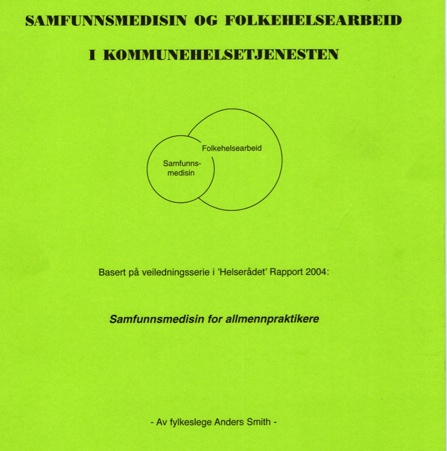
\includegraphics[width=4in]{./andsmi}}%utklipp fra fh profilen 2013
                    	  \captionsetup{singlelinecheck=off}
                      	\caption{Slik ser forsiden ut på en av norges mest undervurderte rapporter}
                      	\label{andsmifig}
                      	%\textit{tjenestetilbudene}.]
                    \end{figure}   


\chapter{Gjennomføring}
	\section{Finansiering}
		\paragraph{}
			Kommuneøkonomien er som kjent relativt stram. For tiltak med mulige langsiktige positive effekter som neppe kan måles på en god måte finnes det lite handlingsrom. Det er derfor godt å se at det gjøres midler tilgjengelig for å satse på for eksempel fysisk aktivitet i et folkehelseperspektiv\ref{faktfhfig}.
					\begin{figure}[h]
                      \centering
                      	\frame{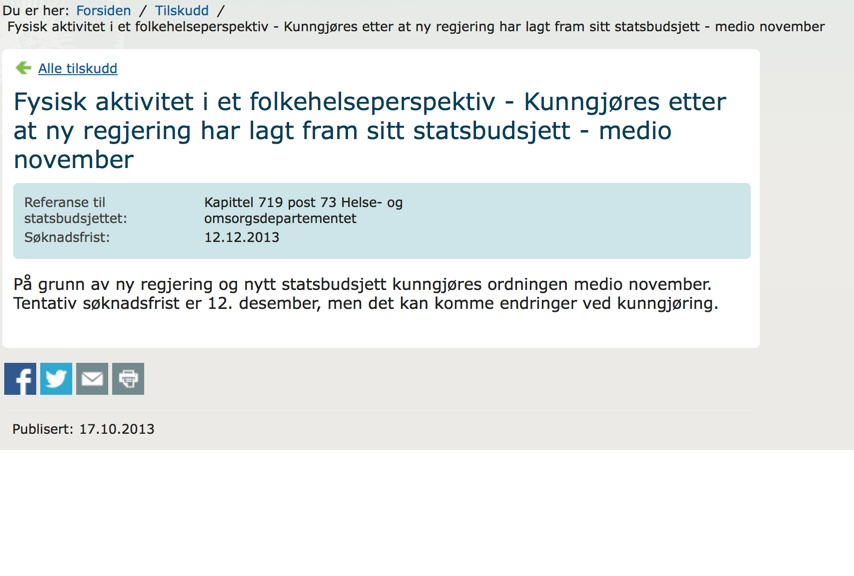
\includegraphics[width=4in]{./faktfh}}%utklipp fra fh profilen 2013
                    	  \captionsetup{singlelinecheck=off}
                      	\caption{Et webutklipp fra tilskuddsportalen til Helsedirektoratet}
                      	\label{faktfhfig}
                      	%\textit{tjenestetilbudene}.]
                    \end{figure}   
        \paragraph{}
            Kommunen har et engasjement i frisklivssentralen som det er viktig å videreføre, men slik situasjonen er nå er vi avhengige av å kunne søke midler. Dette er jo forøvrig en god ting sett fra innbyggernes perspektiv.
	\section{Administrative forutsetninger}
		\paragraph{}
			Her følger en liste med noen punkter som vi har erfart er viktige for å kunne gjennomføre prosjekter slik som dette:
				\begin{itemize}
					\item Målet må være klart formulert. Dette er en forutsetning for at arbeidet skal bli målrettet og alle er på samme side. I tilfellet her vil et mål kunne være: "Gjennom å bruke frisklivssentralen skal man jobbe for å få flere mennesker i alle aldersgrupper i aktivitet i Nedre Eiker. Forprosjektet har som oppgave å utforme en strategi for å kunne tilby aktiviteter til alle grupper i befolkningen. Dette vil være det viktigste tiltaket for å bedre folkehelsa i Nedre Eiker. Strategien skal forankres i kommunestyret og kommunestyret skal være styringsgruppe for prosjektet. Vi ber om et mandat alle politiske partier kan enes om og at dette arbeidet danner ryggraden i folkehelseplanen som er under utarbeidelse."\\
					\item Forankringen må skje i hele orgasisasjonen. Dette er et område hvor prosjektarbeid i tverrfaglige grupper utmerker seg. Bakdelen er at det hersker en ikke ubetydelig prosjekttretthet i kommunen. Det er mange prosjekter og begrenset med tid til møter.\\
					\item Folkehelseplanen må foreligge og implementeres i alt kommunalt plan- og saksarbeid.\\
					\item Frivillige, fastleger og befolkningen må være med å bære prosjektet.\\
				\end{itemize}
	\section{Første skritt på veien}
		\paragraph{}
			Saken må fremmes i H2(Hovedutvalg for helse og omsorg), og det må selges for hva det er: Redningen for folkehelsa i Nedre Eiker. - Dette kan vi ikke operere oss ut av, forteller sykehusdirektør i Helse midt Gunnar Bovim under en presentasjon av Helseundersøkelsen i Nord-Trøndelag(HUNT). Bak ham flimrer en utvikling av overvekt og dermed sykelighet i befolkningen som er skremmende. Dette må formidles helt ned i kommunene og oppgavene må flyttes øverst på dagsorden. Man må forberede seg på en langvarig forpliktelse. Det må befolkningen også.

		\paragraph{}
			Allmennlegen i meg kjenner på håpløsheten i denne monumentale oppgaven, men samfunnsmedisineren kjenner på mulighetene. 

 \renewcommand{\bibname}{Kilder:}
              \begin{thebibliography}{99}

                \bibitem{Stmld47}
                  Helse- og Omsorgsdepartementet,
                  \emph{Stortingsmelding 47, 06/2009, Samhandlindlingsreformen}.
                  Hansen, Bjarne Haakon m. fl. (Minister)

                 \bibitem{fhprofil}
                  Folkehelseprofilen i Nedre Eiker
                  \emph{Folkehelseinstiuttet}.
                  
                  \bibitem{ottawa}
                  Ottawa charter for Health promotion,
                  First International Conference on Health Promotion, Ottawa, 21 November 1986
                  \emph{WHO}.

                  \bibitem{Folkehelseloven}
                  Helse- og Omsorgsdepartementet,
                  \emph{Folkehelseloven, 2012}.
                  Regjeringen Stoltenberg II


                  \bibitem{Utvtrekk}
                  Utviklingstrekkrapport 2010, Folkehelsearbeidet
                  Veien til god helse for alle
                  \emph{Helsedirektoratet IS-1846}.

                  \bibitem{htnorge}
                  Folkehelserapport 2010
                  Helsetilstanden i Norge
                  \emph{Folkehelseinstituttet(FHI)}.

                  \bibitem{aktivhb}
                  Aktivitetshåndboken
                  Helsedirektoratet 2008
                  REDAKTØR: Roald Bahr, prof. dr. med, Norges idrettshøgskole
                 
                  \bibitem{nudge}
                 	Nudge: Improving Decisions About Health, Wealth, and Happiness Paperback
					by Richard H. Thaler (Author) , Cass R. Sunstein  (Author)
                 
                 \bibitem{andsmi}
                  Samfunnsmedisin og folkehelsearbeid i kommunehelsetjenesten
                  Basert på en artikkelserie i Helserådet i 2004
                  \emph{Anders Smith}.

\end{thebibliography}


\end{document}